\documentclass[catalan,a4paper,twoside,11pt]{article}

\usepackage[T1]{fontenc}
\usepackage[utf8]{inputenc}
\DeclareUnicodeCharacter{013F}{\L.}  % ela geminada majúscula
\DeclareUnicodeCharacter{0140}{\l.}  % ela geminada minúscula

\usepackage[widermath]{kpfonts}

\usepackage{beccari-v2}

\usepackage{babel}
\usepackage{varioref}

\usepackage[final]{graphicx}

\usepackage{booktabs}
\usepackage{multicol}

\setlength{\parskip}{1.5ex plus0.5ex minus0.5ex}     % separació entre paràgrafs
\setlength{\parindent}{0mm}

% format de les pàgines
\setlength{\hoffset}{0mm} \setlength{\oddsidemargin}{0mm}
\setlength{\evensidemargin}{-10.8mm} \setlength{\textwidth}{170mm}
\setlength{\marginparsep}{2mm} \setlength{\marginparwidth}{12mm}
\setlength{\voffset}{0mm} \setlength{\textheight}{230mm}
\setlength{\topmargin}{0mm}

\usepackage[pdftex=true,
bookmarks=true,bookmarksopenlevel=0,bookmarksopen=true,bookmarksnumbered=true,
pdftitle={Càlcul Vectorial},pdfauthor={Josep
Mollera},pdfview={FitH},pdfstartview={FitH}, pdfpagelabels=true,
colorlinks=true,linkcolor=black,plainpages=false]{hyperref}


\begin{document}

\title{Càlcul Vectorial en $\mathbb{R}^3$}
\author{Josep Mollera Barriga}
\date{11 de setembre de 2015}
\maketitle



\section{Definicions}

Es dóna  en primer lloc la definició de les variables que s'utilitzen en aquest document.

\begin{list}{}
{\setlength{\labelwidth}{16mm}
\setlength{\leftmargin}{18mm}\setlength{\labelsep}{2mm}}
   \item[$V$:] Volum d'integració.
   \item[$S$:] Superfície d'integració.
   \item[$C$:] Corba d'integració.
   \item[$\diff\tau$:] Diferencial de volum, del volum V.
   \item[$\boldsymbol{\diff a}$:] Vector diferencial de superfície, de la superfície
   $S$. $\boldsymbol{\diff a}$ és perpendicular a $S$.
   \item[$\boldsymbol{\diff l}$:] Vector diferencial de longitud, de la corba
   $C$. $\boldsymbol{\diff l}$ és tangent a $C$.
   \item[$x,y,z$:] Coordenades d'un punt en un sistema de
   coordenades cartesianes.
   \item[$\rho,\phi,z$:] Coordenades d'un punt en un sistema de
   coordenades cilíndriques.
   \item[$r,\theta,\phi$:] Coordenades d'un punt en un sistema de
   coordenades esfèriques.
   \item[$u,v,w$:] Coordenades d'un punt en un sistema de
   coordenades qualssevol.
   \item[$\boldsymbol{\hat{x}},\boldsymbol{\hat{y}},\boldsymbol{\hat{z}}$:]
   Vectors directors d'un sistema de  coordenades
   cartesianes.
   \item[$\boldsymbol{\hat{\rho}},\boldsymbol{\hat{\phi}},\boldsymbol{\hat{z}}$:] Vectors directors d'un sistema de
   coordenades cilíndriques.
   \item[$\boldsymbol{\hat{r}},\boldsymbol{\hat{\theta}},\boldsymbol{\hat{\phi}}$:] Vectors directors d'un sistema de
   coordenades esfèriques.
   \item[$\boldsymbol{\hat{u}},\boldsymbol{\hat{v}},\boldsymbol{\hat{w}}$:]
   Vectors directors d'un sistema de  coordenades
   qualssevol.
   \item[$P, Q$:] Punts en $\mathbb{R}^3$.
   \item[$\boldsymbol{A,B,C}$:] Vectors en $\mathbb{R}^3$.
   \item[$\alpha$:] Angle entre dos vectors en $\mathbb{R}^3$.
   \item[$f,g$:] Funcions escalars.\hspace{1mm} $f,g \colon \mathbb{R}^3\rightarrow\mathbb{R}$.
   \item[$\boldsymbol{F,G}$:] Funcions vectorials. \hspace{1mm} $\boldsymbol{F,G}\colon\mathbb{R}^3\rightarrow\mathbb{R}^3$.
   \item[$\boldsymbol{\nabla}f$:] Gradient de la funció escalar $f$. \hspace{1mm}
   $\boldsymbol{\nabla}f\colon\mathbb{R}\rightarrow\mathbb{R}^3$
   \item[$\boldsymbol{\nabla\cdot F}$:] Divergència de la funció vectorial $\boldsymbol{F}$. \hspace{1mm}
   $\boldsymbol{\nabla\cdot F}\colon \mathbb{R}^3\rightarrow\mathbb{R}$.
   \item[$\boldsymbol{\nabla\times F}$:] Rotacional de la funció vectorial $\boldsymbol{F}$. \hspace{1mm}
   $\boldsymbol{\nabla\times F}\colon   \mathbb{R}^3\rightarrow\mathbb{R}^3$.
   \item[$\boldsymbol{\nabla^2}f$:] Laplacià de la funció escalar $f$. \hspace{1mm}
   $\boldsymbol{\nabla^2}f\colon \mathbb{R}\rightarrow\mathbb{R}$.
   \item[$\boldsymbol{\nabla^2F}$:] Laplacià de la funció vectorial $\boldsymbol{F}$. \hspace{1mm} $\boldsymbol{\nabla^2F}\colon \mathbb{R}^3\rightarrow\mathbb{R}^3$.
\end{list}

\newcommand{\va}{\ensuremath{\,\boldsymbol{\hat{x}}}}
\newcommand{\vb}{\ensuremath{\,\boldsymbol{\hat{y}}}}
\newcommand{\vc}{\ensuremath{\,\boldsymbol{\hat{z}}}}
\section{Sistemes de Coordenades}

Es representen en la Figura \vref{pic:coord-cart-cil-esf}, tres dels
sistemes de coordenades més utilitzats: el cartesià, el
cilíndric i l'esfèric.

En el sistema de coordenades cartesianes, els vectors directors
tenen una orientació fixa, mentre que en els sistemes de
coordenades cilíndriques i esfèriques, els vectors
directors tenen una orientació variable, que depèn del punt
$P$ al qual ens estiguem referint.


\begin{figure}[h]
\centering
   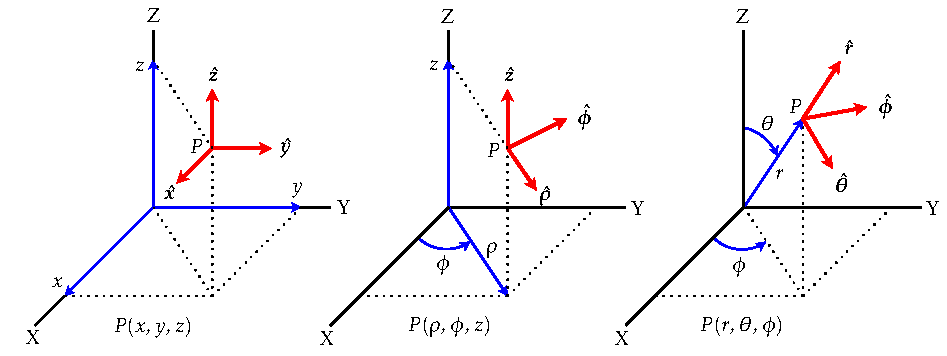
\includegraphics{Imatges/Coordenades.pdf}
\caption{Coordenades cartesianes, cilíndriques i esfèriques}
\label{pic:coord-cart-cil-esf}
\end{figure}

En la Taula \vref{taula:coord} es donen els rangs de les coordenades de cadascun d'aquests tres sistemes.
\begin{table}[htb]
   \caption{\label{taula:coord}Rangs de les Coordenades}
   \[ \begin{array}{lllll}
   \toprule[1pt]
   \text{Cartesianes} &  & \text{Cilíndriques} & & \text{Esfèriques}
   \\
   \midrule
      x\in(-\infty,\infty) &   & \rho\in[0,\infty)    &  &  r\in[0,\infty)  \\
      y\in(-\infty,\infty) &   & \phi\in[0,2\pi)   &  &  \theta\in[0,\pi] \\
      z\in(-\infty,\infty) &   & z\in(-\infty,\infty) &  &  \phi\in[0,2\pi) \\
   \bottomrule[1pt]
   \end{array}   \]
\end{table}

\subsection{Relacions entre les coordenades cartesianes i
cilíndriques}

Les coordenades cartesianes  d'un punt $P(x,y,z)$, s'obtenen a partir
de les seves coordenades cilíndriques $P(\rho,\phi,z)$,
mitjançant les relacions següents:
\begin{subequations}\begin{align}
    x &=\rho\cos\phi \\ y &=\rho\sin\phi \\ z &=z
\end{align}\end{subequations}

Les coordenades  cilíndriques  d'un punt $P(\rho,\phi,z)$,
s'obtenen a partir de les seves coordenades cartesianes $P(x,y,z)$,
mitjançant les relacions següents:
\begin{subequations}\begin{align}
    \rho &= \sqrt{x^2+y^2}\\
    \phi &=  \arctan\frac{y}{x}\\
    z &= z
\end{align}\end{subequations}

L'expressió en coordenades cartesianes dels vectors directors d'un sistema de coordenades  cilíndriques $\boldsymbol{\hat{\rho}},\boldsymbol{\hat{\phi}},\boldsymbol{\hat{z}}$, en un punt $P(\rho,\phi,z)$ donat en coordenades cilíndriques, és:
\begin{subequations}\begin{align}
    \boldsymbol{\hat{\rho}} &=\cos\phi\va+\sin\phi\vb \\
    \boldsymbol{\hat{\phi}} &=-\sin\phi\va+\cos\phi\vb \\
    \boldsymbol{\hat{z}} &=\vc
\end{align}\end{subequations}

L'expressió en coordenades cilíndriques dels vectors directors d'un sistema de coordenades  cartesianes $\va,\vb,\vc$, en un punt $P(\rho,\phi,z)$ donat en coordenades cilíndriques, és:
\begin{subequations}\begin{align}
    \va &=\cos\phi\,\boldsymbol{\hat{\rho}}-\sin\phi\,\boldsymbol{\hat{\phi}} \\
    \vb &=\sin\phi\,\boldsymbol{\hat{\rho}}+\cos\phi\,\boldsymbol{\hat{\phi}} \\
    \vc &=\boldsymbol{\hat{z}}
\end{align}\end{subequations}

Les components d'un vector en coordenades cartesianes ($A_x, A_y, A_z)$, s'obtenen a partir de les seves components en coordenades cilíndriques $(A_\rho, A_\phi, A_z)$, en un punt $P(\rho,\phi,z)$ donat en coordenades cilíndriques, mitjançant les relacions següents:
\begin{subequations}\begin{align}
    A_x &=A_\rho \cos\phi -A_\phi\sin\phi \\
    A_y &=A_\rho\sin\phi +A_\phi\cos\phi\\
    A_z &= A_z
\end{align}\end{subequations}

Les components d'un vector en coordenades cilíndriques $(A_\rho, A_\phi, A_z)$, s'obtenen a partir de les seves components en coordenades cartesianes ($A_x, A_y, A_z)$, en un punt $P(\rho,\phi,z)$ donat en coordenades cilíndriques, mitjançant les relacions següents:
\begin{subequations}\begin{align}
    A_\rho &=  A_x\cos\phi+A_y\sin\phi\\
    A_\phi &= -A_x\sin\phi+A_y\cos\phi \\
    A_z &= A_z
\end{align}\end{subequations}


\subsection{Relacions entre les coordenades cartesianes i
esfèriques}

Les coordenades cartesianes  d'un punt $P(x,y,z)$, s'obtenen a partir
de les seves coordenades esfèriques $P(r,\theta,\phi)$,
mitjançant les relacions següents:
\begin{subequations}\begin{align}
    x &=r\sin\theta\cos\phi \\ y &=r\sin\theta\sin\phi \\ z &=r\cos\theta
\end{align}\end{subequations}

Les coordenades  esfèriques  d'un punt $P(r,\theta,\phi)$,
s'obtenen a partir de les seves coordenades cartesianes $P(x,y,z)$,
mitjançant les relacions següents:
\begin{subequations}\begin{align}
    r &=\sqrt{x^2+y^2+z^2}\\
    \theta&=\arccos\frac{z}{\sqrt{x^2+y^2+z^2}}\\[1mm]
    \phi &=\arctan\frac{y}{x}
\end{align}\end{subequations}


L'expressió en coordenades cartesianes dels vectors directors d'un sistema de coordenades  esfèriques $\boldsymbol{\hat{r}},\boldsymbol{\hat{\theta}},\boldsymbol{\hat{\phi}}$, en un punt $P(r,\theta,\phi)$ donat en coordenades esfèriques, és:
\begin{subequations}\begin{align}
    \boldsymbol{\hat{r}} &=\sin\theta\cos\phi\va+ \sin\theta\sin\phi\vb+\cos\theta\vc\\
    \boldsymbol{\hat{\theta}} &=\cos\theta\cos\phi\va+
    \cos\theta\sin\phi\vb-\sin\theta\vc\\
    \boldsymbol{\hat{\phi}}&=-\sin\phi\va+\cos\phi\vb
\end{align}\end{subequations}

L'expressió en coordenades esfèriques dels vectors directors d'un sistema de coordenades  cartesianes $\va,\vb,\vc$, en un punt $P(r,\theta,\phi)$ donat en coordenades esfèriques, és:
\begin{subequations}\begin{align}
    \va &=\sin\theta\cos\phi\,\boldsymbol{\hat{r}}+
    \cos\theta\cos\phi\,\boldsymbol{\hat{\theta}}-\sin\phi\,\boldsymbol{\hat{\phi}}\\
    \vb &=\sin\theta\sin\phi\,\boldsymbol{\hat{r}}+
    \cos\theta\sin\phi\,\boldsymbol{\hat{\theta}}+\cos\phi\,\boldsymbol{\hat{\phi}}\\
    \vc &=\cos\theta\,\boldsymbol{\hat{r}}-\sin\theta\,\boldsymbol{\hat{\theta}}
\end{align}\end{subequations}

Les components d'un vector en coordenades cartesianes $(A_x, A_y, A_z)$, s'obtenen a partir de les seves components en coordenades esfèriques $(A_r, A_\theta, A_\phi)$, en un punt $P(r,\theta,\phi)$ donat en coordenades esfèriques, mitjançant les relacions següents:
\begin{subequations}\begin{align}
    A_x &= A_r\sin\theta\cos\phi+A_\theta\cos\theta\cos\phi-A_\phi\sin\phi \\
    A_y &= A_r\sin\theta\sin\phi+A_\theta\cos\theta\sin\phi+A_\phi\cos\phi\\
    A_z &= A_r\cos\theta-A_\theta\sin\theta
\end{align}\end{subequations}

Les components d'un vector en coordenades esfèriques $(A_r, A_\theta, A_\phi)$, s'obtenen a partir de les seves components en coordenades cartesianes $(A_x, A_y, A_z)$, en un punt $P(r,\theta,\phi)$ donat en coordenades esfèriques, mitjançant les relacions següents:
\begin{subequations}\begin{align}
    A_r &=  A_x\sin\theta\cos\phi+A_y\sin\theta\sin\phi+A_z\cos\theta\\
    A_\theta &=  A_x\cos\theta\cos\phi+A_y\cos\theta\sin\phi-A_z\sin\theta\\
    A_\phi &= -A_x\sin\phi+A_y\cos\phi
\end{align}\end{subequations}


\subsection{Relacions entre les coordenades cilíndriques i
esfèriques}

Les coordenades cilíndriques  d'un punt $P(\rho,\phi,z)$,
s'obtenen a partir de les seves coordenades esfèriques
$P(r,\theta,\phi)$, mitjançant les relacions següents:
\begin{subequations}\begin{align}
    \rho &=r\sin\theta \\ \phi &=\phi \\z &=r\cos\theta
\end{align}\end{subequations}

Les coordenades  esfèriques  d'un punt $P(r,\theta,\phi)$,
s'obtenen a partir de les seves coordenades cilíndriques
$P(\rho,\phi,z)$, mitjançant les relacions següents:
\begin{subequations}\begin{align}
    r &=\sqrt{\rho^2+z^2}\\
    \theta &=\arctan\frac{\rho}{z}\\
    \phi &=\phi
\end{align}\end{subequations}

L'expressió en coordenades cilíndriques dels vectors directors d'un sistema de coordenades  esfèriques $\boldsymbol{\hat{r}},\boldsymbol{\hat{\theta}},\boldsymbol{\hat{\phi}}$, en un punt $P(r,\theta,\phi)$ donat en coordenades esfèriques, és:
\begin{subequations}\begin{align}
    \boldsymbol{\hat{r}} &=\sin\theta\,\boldsymbol{\hat{\rho}}+\cos\theta\,\boldsymbol{\hat{z}}\\
    \boldsymbol{\hat{\theta}}
    &=\cos\theta\,\boldsymbol{\hat{\rho}}-\sin\theta\,\boldsymbol{\hat{z}}\\
    \boldsymbol{\hat{\phi}}&=\boldsymbol{\hat{\phi}}
\end{align}\end{subequations}

L'expressió en coordenades esfèriques dels vectors directors d'un sistema de coordenades  cilíndriques $\boldsymbol{\hat{\rho}},\boldsymbol{\hat{\phi}},\boldsymbol{\hat{\theta}}$, en un punt $P(r,\theta,\phi)$ donat en coordenades esfèriques, és:
\begin{subequations}\begin{align}
    \boldsymbol{\hat{\rho}} &=\sin\theta\,\boldsymbol{\hat{r}}+
    \cos\theta\,\boldsymbol{\hat{\theta}}\\
    \boldsymbol{\hat{\phi}}&=\boldsymbol{\hat{\phi}}\\
    \boldsymbol{\hat{z}} &=\cos\theta\,\boldsymbol{\hat{r}}-
    \sin\theta\,\boldsymbol{\hat{\theta}}
\end{align}\end{subequations}

Les components d'un vector en coordenades cilíndriques  $(A_\rho, A_\phi, A_z)$, s'obtenen a partir de les seves components en coordenades esfèriques $(A_r, A_\theta, A_\phi)$, en un punt $P(r,\theta,\phi)$ donat en coordenades esfèriques, mitjançant les relacions següents:
\begin{subequations}\begin{align}
    A_\rho &= A_r\sin\theta+A_\theta\cos\theta \\
    A_\phi &= A_\phi\\
    A_z &= A_r\cos\theta-A_\theta\sin\theta
\end{align}\end{subequations}

Les components d'un vector en coordenades esfèriques $(A_r, A_\theta, A_\phi)$, s'obtenen a partir de les seves components en coordenades cilíndriques $(A_\rho, A_\phi, A_z)$, en un punt $P(r,\theta,\phi)$ donat en coordenades esfèriques, mitjançant les relacions següents:
\begin{subequations}\begin{align}
    A_r &=  A_\rho\sin\theta+A_z\cos\theta\\
    A_\theta &=  A_\rho\cos\theta-A_z\sin\theta\\
    A_\phi &= A_\phi
\end{align}\end{subequations}


\section{Operacions  Bàsiques}
\renewcommand{\va}{\ensuremath{\,\boldsymbol{\hat{u}}}}
\renewcommand{\vb}{\ensuremath{\,\boldsymbol{\hat{v}}}}
\renewcommand{\vc}{\ensuremath{\,\boldsymbol{\hat{w}}}}

A partir de les components $(A_u,A_v,A_w)$ i $(B_u,B_v,B_w)$
de dos vectors $\boldsymbol{A}$ i $\boldsymbol{B}$, tenim:

\subsection{Mòdul}
\vspace{-5mm}
\begin{equation}
    |\boldsymbol{A}|=  \sqrt{A_u^2 + A_v^2 + A_w^2}
\end{equation}

\subsection{Addició i substracció}
\vspace{-5mm}
\begin{subequations}\begin{align}
    \boldsymbol{A+B}= (A_u+B_u)\va + (A_v+B_v)\vb + (A_w+B_w)\vc \\
    \boldsymbol{A-B}= (A_u-B_u)\va + (A_v-B_v)\vb + (A_w-B_w)\vc
\end{align}\end{subequations}

\subsection{Producte escalar}
\vspace{-5mm}
\begin{align}
    \boldsymbol{A\cdot B} &= A_u B_u + A_v B_v + A_w B_w\\
    \boldsymbol{A\cdot B} &=|\boldsymbol{A}| \, |\boldsymbol{B}| \cos\alpha\\
    \boldsymbol{A\cdot B} &=\boldsymbol{B\cdot A}\\
    \boldsymbol{A\cdot(B+C)} &= \boldsymbol{A\cdot B+ A\cdot C}
\end{align}

El producte escalar de dos vectors perpendiculars  és nul.

\subsection{Producte vectorial}
\vspace{-5mm}
\begin{align}
    \boldsymbol{A\times B} &= (A_v B_w - A_w B_v)\va + (A_w B_u - A_u B_w)\vb +
    (A_u B_v - A_v B_u)\vc \\
    |\boldsymbol{A\times B}| &=|\boldsymbol{A}| \, |\boldsymbol{B}| \sin\alpha\\
    \boldsymbol{A\times B} &=-(\boldsymbol{B\times A})\\
    \boldsymbol{A\times(B+C)} &= \boldsymbol{A\times B+ A\times C}
\end{align}

El producte vectorial de dos vectors paraŀlels  és nul.

El producte vectorial de dos vectors és un altre vector, el
sentit del qual ve donat per la regla del cargol: és el sentit
d'avanç que té un cargol, amb el seu eix perpendicular al
pla format pels vectors  $\boldsymbol{A}$ i $\boldsymbol{B}$, quan
gira en el sentit que portaria el primer vector  $\boldsymbol{A}$ a
trobar el segon vector $\boldsymbol{B}$, utilitzant el menor angle
possible.

\subsection{Derivada temporal}
\begin{equation}
    \deriv{\boldsymbol{A}}{t} = \deriv{A_u}{t}\va +
    \deriv{A_v}{t}\vb + \deriv{A_w}{t}\vc
\end{equation}


\section{Càlcul Diferencial }

\subsection{Coordenades cartesianes}
\renewcommand{\va}{\ensuremath{\,\boldsymbol{\hat{x}}}}
\renewcommand{\vb}{\ensuremath{\,\boldsymbol{\hat{y}}}}
\renewcommand{\vc}{\ensuremath{\,\boldsymbol{\hat{z}}}}

Es donen a continuació les derivades parcials dels vectors directors $\va$, $\vb$ i $\vc$, respecte $x$, $y$ i $z$:
\begin{subequations}
\begin{align}
   \pderiv{\va}{x} &= 0 & \pderiv{\va}{y} &= 0 & \pderiv{\va}{z} &= 0 \\
   \pderiv{\vb}{x} &= 0 & \pderiv{\vb}{y} &= 0 & \pderiv{\vb}{z} &= 0 \\
   \pderiv{\vc}{x} &= 0 & \pderiv{\vc}{y} &= 0 & \pderiv{\vc}{z} &= 0
\end{align}
\end{subequations}

En les equacions següents, $(F_x,F_y,F_z)$  són les
components de la funció  vectorial $\boldsymbol{F}$ en un sistema de
coordenades cartesianes. En aquestes coordenades tenim:
\begin{align}
    \boldsymbol{\diff l} &= \diff x \va + \diff y \vb + \diff z \vc\\[1ex]
    \boldsymbol{\diff a} &= \diff x \diff y \vc \qquad\text{(en un pla
    paraŀlel a l'X-Y)}\\[1ex]
    \boldsymbol{\diff a} &= \diff x \diff z \vb \qquad\text{ (en un pla
    paraŀlel a l'X-Z)}\\[1ex]
    \boldsymbol{\diff a} &= \diff y \diff z \va \qquad\text{ (en un pla
    paraŀlel a l'Y-Z)}\\[1ex]
    \diff\tau &= \diff x \diff y \diff z\\[1ex]
    \boldsymbol{\nabla}f &= \pderiv{f}{x}\va + \pderiv{f}{y}\vb
    + \pderiv{f}{z}\vc\\[1ex]
    \boldsymbol{\nabla\cdot F} &= \pderiv{F_x}{x} + \pderiv{F_y}{y}
    + \pderiv{F_z}{z}\\[1ex]
    \boldsymbol{\nabla\times F} &= \left[\pderiv{F_z}{y}-\pderiv{F_y}{z}\right]\va +
    \left[\pderiv{F_x}{z}-\pderiv{F_z}{x}\right]\vb +
    \left[\pderiv{F_y}{x}-\pderiv{F_x}{y}\right]\vc\\[1ex]
    \boldsymbol{\nabla^2}f &= \pderiv[2]{f}{x} + \pderiv[2]{f}{y}+ \pderiv[2]{f}{z}
\end{align}

\subsection{Coordenades cilíndriques}

\renewcommand{\va}{\ensuremath{\,\boldsymbol{\hat{\rho}}}}
\renewcommand{\vb}{\ensuremath{\,\boldsymbol{\hat{\phi}}}}
\renewcommand{\vc}{\ensuremath{\,\boldsymbol{\hat{z}}}}

Es donen a continuació les derivades parcials dels vectors directors $\va$, $\vb$ i $\vc$, respecte $\rho$, $\phi$ i $z$:
\begin{subequations}
\begin{align}
   \pderiv{\va}{\rho} &= 0 & \pderiv{\va}{\phi} &= \vb  & \pderiv{\va}{z} &= 0 \\
   \pderiv{\vb}{\rho} &= 0 & \pderiv{\vb}{\phi} &= -\va & \pderiv{\vb}{z} &= 0 \\
   \pderiv{\vc}{\rho} &= 0 & \pderiv{\vc}{\phi} &= 0    & \pderiv{\vc}{z} &= 0
\end{align}
\end{subequations}

En les equacions següents, $(F_\rho,F_\phi,F_z)$  són les
components de la funció vectorial   $\boldsymbol{F}$ en un sistema de
coordenades cilíndriques. En aquestes coordenades tenim:
\begin{align}
    \boldsymbol{\diff l} &= \diff \rho \va + \rho\diff \phi \vb + \diff z \vc\\[1ex]
    \boldsymbol{\diff a} &= \rho\diff \phi \diff z \va\qquad\text{(en una superfície cilíndrica)}\\[1ex]
    \diff\tau &= \rho \diff \rho \diff \phi \diff z\\[1ex]
    \boldsymbol{\nabla}f &= \pderiv{f}{\rho}\va + \frac{1}{\rho}\pderiv{f}{\phi}\vb
    + \pderiv{f}{z}\vc\\[1ex]
    \boldsymbol{\nabla\cdot F} &= \frac{1}{\rho}\pderiv{}{\rho}(\rho F_\rho) +
    \frac{1}{\rho}\pderiv{F_\phi}{\phi}+ \pderiv{F_z}{z}\\[1ex]
    \boldsymbol{\nabla\times F} &= \left[\frac{1}{\rho}\pderiv{F_z}{\phi}-
    \pderiv{F_\phi}{z}\right]\va +
    \left[\pderiv{F_\rho}{z}-\pderiv{F_z}{\rho}\right]\vb +
    \frac{1}{\rho}\left[\pderiv{}{\rho}(\rho F_\phi)-\pderiv{F_\rho}{\phi}\right]\vc\\[1ex]
    \boldsymbol{\nabla^2}f &= \frac{1}{\rho}\pderiv{}{\rho}\left(\rho\pderiv{f}{\rho}
    \right)
    + \frac{1}{\rho^2}\pderiv[2]{f}{\phi}+ \pderiv[2]{f}{z}
\end{align}


\subsection{Coordenades esfèriques}

\renewcommand{\va}{\ensuremath{\,\boldsymbol{\hat{r}}}}
\renewcommand{\vb}{\ensuremath{\,\boldsymbol{\hat{\theta}}}}
\renewcommand{\vc}{\ensuremath{\,\boldsymbol{\hat{\phi}}}}

Es donen a continuació les derivades parcials dels vectors directors $\va$, $\vb$ i $\vc$, respecte  $r$, $\theta$ i $\phi$:
\begin{subequations}
\begin{align}
   \pderiv{\va}{r} &= 0 & \pderiv{\va}{\theta} &= \vb  & \pderiv{\va}{\phi} &= \sin\theta\vc \\
   \pderiv{\vb}{r} &= 0 & \pderiv{\vb}{\theta} &= -\va & \pderiv{\vb}{\phi} &= \cos\theta\vc \\
   \pderiv{\vc}{r} &= 0 & \pderiv{\vc}{\theta} &= 0    & \pderiv{\vc}{\phi} &= -\sin\theta\va-\cos\theta\vb
\end{align}
\end{subequations}

En les equacions següents, $(F_r,F_\theta,F_\phi)$  són
les components de la funció  vectorial  $\boldsymbol{F}$ en un sistema de
coordenades esfèriques. En aquestes coordenades tenim:
\begin{align}
    \boldsymbol{\diff l} &= \diff r \va + r\diff\theta \vb + r \sin\theta\diff \phi \vc\\[1ex]
    \boldsymbol{\diff a} &= r^2 \sin\theta \diff \theta \diff \phi \va\qquad\text{(en una superfície esfèrica)}\\[1ex]
    \diff\tau &= r^2 \sin\theta\diff r \diff \theta \diff \phi\\[1ex]
    \boldsymbol{\nabla}f &= \pderiv{f}{r}\va + \frac{1}{r}\pderiv{f}{\theta}\vb
    + \frac{1}{r\sin\theta}\pderiv{f}{\phi}\vc\\[1ex]
    \boldsymbol{\nabla\cdot F} &= \frac{1}{r^2}\pderiv{}{r}(r^2 F_r) +
    \frac{1}{r\sin\theta}\pderiv{}{\theta}(F_\theta\sin\theta)+
    \frac{1}{r\sin\theta}\pderiv{F_\phi}{\phi}\\[1ex]
    \boldsymbol{\nabla\times F} &= \frac{1}{r\sin\theta}\left[\pderiv{}{\theta}
    (F_\phi\sin\theta)-\pderiv{F_\theta}{\phi}\right]\va +
    \frac{1}{r}\left[\frac{1}{\sin\theta}\pderiv{F_r}{\phi}-
    \pderiv{}{r}(r F_\phi)\right]\vb +\frac{1}{r}\left[\pderiv{}{r}(r F_\theta)-\pderiv{F_r}{\theta}\right]\vc\\[1ex]
    \boldsymbol{\nabla^2}f &= \frac{1}{r^2}\pderiv{}{r}\left(r^2\pderiv{f}{r}
    \right) + \frac{1}{r^2\sin\theta}\pderiv{}{\theta}\left(\sin\theta\pderiv{f}{\theta}\right) +
    \frac{1}{r^2\sin^2\theta}\pderiv[2]{f}{\phi}
\end{align}


\section{Relacions}

\subsection{Operadors}
\renewcommand{\va}{\ensuremath{\,\boldsymbol{\hat{x}}}}
\renewcommand{\vb}{\ensuremath{\,\boldsymbol{\hat{y}}}}
\renewcommand{\vc}{\ensuremath{\,\boldsymbol{\hat{z}}}}
Els operadors $\boldsymbol{\nabla}$ i $\boldsymbol{\nabla^2}$ es defineixen en coordenades cartesianes, segons les relacions següents:
\begin{align}
    \boldsymbol{\nabla} &\equiv \va \pderiv{}{x} + \vb \pderiv{}{y}
    + \vc \pderiv{}{z}\\[0.5ex]
    \boldsymbol{\nabla^2} &\equiv \pderiv[2]{}{x} + \pderiv[2]{}{y}+ \pderiv[2]{}{z}
\end{align}

\subsection{Identitats}
Es compleixen les identitats següents:
\begin{align}
    \boldsymbol{\nabla^2}f &=\boldsymbol{\nabla\cdot}(\boldsymbol{\nabla}f)\\
    \boldsymbol{\nabla^2 F}  &= \boldsymbol{\nabla}(\boldsymbol{\nabla\cdot F})
    - \boldsymbol{\nabla\times}(\boldsymbol{\nabla\times F})\\
    \boldsymbol{\nabla\times}(\boldsymbol{\nabla}f) &= 0\\
    \boldsymbol{\nabla\cdot}(\boldsymbol{\nabla\times F}) &= 0
\end{align}

\subsection{Gradient}
El gradient compleix les relacions següents:
\begin{align}
    \boldsymbol{\nabla}(f+g) &= \boldsymbol{\nabla}f + \boldsymbol{\nabla}g\\
    \boldsymbol{\nabla}(fg) &= f \boldsymbol{\nabla}g + g \boldsymbol{\nabla} f\\
    \boldsymbol{\nabla}(\boldsymbol{F\cdot G}) &=
    \boldsymbol{F\times}(\boldsymbol{\nabla\times G}) + \boldsymbol{G\times}(\boldsymbol{\nabla\times F}) +
    (\boldsymbol{F\cdot\nabla})\boldsymbol{G} + (\boldsymbol{G\cdot\nabla})\boldsymbol{F}
\end{align}

\subsection{Divergència}
La divergència compleix les relacions següents:
\begin{align}
    \boldsymbol{\nabla\cdot}(\boldsymbol{A}+\boldsymbol{B}) &= (\boldsymbol{\nabla\cdot A}) +
    (\boldsymbol{\nabla\cdot B})\\
    \boldsymbol{\nabla\cdot}(f\boldsymbol{F}) &=
    (\boldsymbol{\nabla}f)\boldsymbol{\cdot F} + f(\boldsymbol{\nabla\cdot F})\\
       \boldsymbol{\nabla\cdot}(\boldsymbol{F\times G}) &=
    \boldsymbol{G\cdot}(\boldsymbol{\nabla\times F}) -
    \boldsymbol{F\cdot}(\boldsymbol{\nabla\times G})
\end{align}

\subsection{Rotacional}
El rotacional compleix les relacions següents:
\begin{align}
    \boldsymbol{\nabla\times}(\boldsymbol{A}+\boldsymbol{B}) &= (\boldsymbol{\nabla\times A}) + (\boldsymbol{\nabla\times B})\\
    \boldsymbol{\nabla\times}(f\boldsymbol{F}) &=
    (\boldsymbol{\nabla}f)\boldsymbol{\times F} + f(\boldsymbol{\nabla\times F})\\
    \boldsymbol{\nabla\times}(\boldsymbol{F\times G}) &= (\boldsymbol{G\cdot\nabla})\boldsymbol{F} - (\boldsymbol{F\cdot\nabla})\boldsymbol{G} + \boldsymbol{F}(\boldsymbol{\nabla\cdot G}) - \boldsymbol{G}(\boldsymbol{\nabla\cdot F})
\end{align}


\section{Teoremes Vectorials}

La funció escalar $f$ i la funció vectorial $\boldsymbol{F}$ que apareixen en els teoremes següents han de ser contínues, diferenciables i les seves derivades primeres han de ser funcions contínues.

\subsection{Teorema fonamental del gradient}
Estableix que la integral sobre una corba $C$ de la funció $\boldsymbol{\nabla} f$ només depèn dels punts inicial i final sobre la corba, $P$ i $Q$, i no del camí seguit per anar de l'un a l'altre.
\begin{equation}
    \varint_{C_{P\rightarrow Q}} (\boldsymbol{\nabla}f) \cdot \diff l = f(Q)-f(P)
\end{equation}

Evidentment, la integral anterior és nuŀla quan la corba d'integració és tancada ($P \equiv Q$).
\begin{equation}
    \oint_C (\boldsymbol{\nabla}f) \cdot \diff l = 0
\end{equation}

\subsection{Teorema fonamental de la divergència (també anomenat de Gauss o de Green)}
Estableix la relació entre la integral sobre un volum $V$ de la funció $\boldsymbol{\nabla\cdot F}$ i la integral sobre una superfície $S$ de la funció $\boldsymbol{F}$, on $S$ és la superfície tancada que limita $V$.
\begin{equation}
    \variiint_V(\boldsymbol{\nabla\cdot F})\,\diff \tau = \oiint_S\boldsymbol{F\cdot\diff a}
\end{equation}

El vector $\boldsymbol{\diff a}$ apunta sempre cap a fora del volum $V$.

\subsection{Teorema fonamental del rotacional (també anomenat d'Stokes)}
Estableix la relació entre la integral sobre una superfície $S$ de la funció $\boldsymbol{\nabla\times F}$ i la integral sobre una corba $C$ de la funció $\boldsymbol{F}$, on $C$ és la corba tancada que limita $S$.
\begin{equation}
    \variint_S(\boldsymbol{\nabla\times F})\boldsymbol{\,\cdot\diff a} =
    \oint_C\boldsymbol{F\cdot\diff l}
\end{equation}

D'aquesta relació es desprèn que la integral de $\boldsymbol{\nabla\times F}$ sobre qualsevol superfície $S$ limitada per la mateixa corba $C$, té el mateix valor.

Evidentment, la integral anterior és nuŀla quan la superfície d'integració és tancada.
\begin{equation}
    \oiint_S(\boldsymbol{\nabla\times F})\boldsymbol{\,\cdot\diff a} = 0
\end{equation}

En la Figura \vref{pic:signe-teo-stockes} s'iŀlustra el conveni de
signes dels vectors $\boldsymbol{\diff l}$ i $\boldsymbol{\diff a}$.

\begin{figure}[h]
\centering
     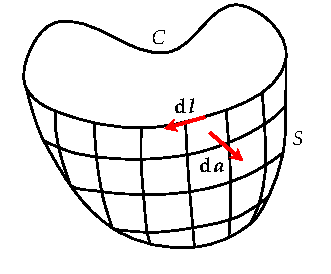
\includegraphics{Imatges/Stokes.pdf}
\caption{Conveni de signes del teorema d'Stokes}
\label{pic:signe-teo-stockes}
\end{figure}


\subsection{Teorema del gradient}
Estableix la relació entre la integral sobre un volum $V$ de la funció $\boldsymbol{\nabla}f$ i la integral sobre una superfície $S$ de la funció $f$, on $S$ és la superfície tancada que limita $V$.
\begin{equation}
    \variiint_V(\boldsymbol{\nabla}f)\diff \tau = \oiint_S f\boldsymbol{\diff a}
\end{equation}

El vector $\boldsymbol{\diff a}$ apunta sempre cap a fora del volum $V$.

\subsection{Teorema del rotacional}
Estableix la relació entre la integral sobre un volum $V$ de la funció $\boldsymbol{\nabla\times F}$ i la integral sobre una superfície $S$ de la funció $\boldsymbol{F}$, on $S$ és la superfície tancada que limita $V$.
\begin{equation}
    \variiint_V(\boldsymbol{\nabla\times F})\,\diff \tau=-\oiint_S
    \boldsymbol{F\times\diff a}
\end{equation}

El vector $\boldsymbol{\diff a}$ apunta sempre cap a fora del volum $V$.

\section{Bibliografia}

\textsc{H. M. Schey}. \textsl{Div, grad curl and all that, an informal text on vector calculus}.  W. W. Norton and Company, 3rd edition, 1997.

\textsc{Paul Lorrain, Dale R. Corson}. \textsl{Electromagnetic fields and waves}.  W. H. Freeman and Company, 1972.

\textsc{David J. Griffiths, Reed College}. \textsl{Introduction to electrodynamics}. Prentice-Hall, 3rd edition, 1999.

\textsc{Daniel Fleisch}. \textsl{A student's guide to Maxwell's equations}. Cambridge University Press, 2008.


\end{document}
